\documentclass[a4paper,parskip=half*,DIV=7,fontsize=11pt]{scrartcl}
\usepackage[T1]{fontenc}
\usepackage[head=27.2pt]{geometry}
\usepackage[english,ngerman]{babel}
\usepackage[utf8]{luainputenc}
\usepackage{amsmath}
\usepackage{amssymb}
\usepackage{amsthm}
\usepackage{mathtools}
\usepackage{scrlayer-scrpage}
\usepackage{braket}
\usepackage{listings}
\usepackage{lastpage}
\usepackage{hyperref}
\usepackage[table]{xcolor}
\usepackage{array}
\usepackage{adjustbox}
\usepackage[basic]{complexity}

\usepackage{pifont}
\newcommand{\cmark}{\text{\ding{51}}}
\newcommand{\xmark}{\text{\ding{55}}}

\DeclarePairedDelimiter\goedel{\langle}{\rangle}

\newcommand\comp[1]{\overline#1}

\lstset{
    mathescape=true
}

\newcommand{\defeq}{\vcentcolon =}
\newcommand{\eqdef}{=\vcentcolon}

\newcommand\blfootnote[1]{%
  \begingroup
  \renewcommand\thefootnote{}\footnote{#1}%
  \addtocounter{footnote}{-1}%
  \endgroup
}

\renewcommand{\arraystretch}{1.2}
\newcolumntype{L}{>{$}l<{$}}

\ihead{BuK Panikzettel}
\title{BuK Panikzettel}
\author{Luca Oeljeklaus, der Dude\blfootnote{Pseudonyme geh\"oren anonymen Autoren, die anonym bleiben wollen.}, Caspar Zecha,\\ Tobias Polock, Philipp Schröer}
\cfoot{\thepage\ / \pageref{LastPage}}

\lstset{basicstyle=\ttfamily}

\begin{document}

\maketitle

\begin{abstract}
Dieser Panikzettel ist über die Vorlesung Berechenbarkeit und Komplexität. Er basiert auf dem Foliensatz von Prof. Dr. Pascal Schweitzer aus dem Wintersemester 16/17.	\\
Dieser Panikzettel ist Open Source. Wir freuen uns über Anmerkungen und Verbesserungsvorschläge auf \url{https://git.rwth-aachen.de/philipp.schroer/panikzettel}.
\end{abstract}

\tableofcontents

\newpage

\section{Einleitung}

Wir haben uns entschieden, nur die wichtigsten Ergebnisse der Vorlesung hier im Panikzettel zusammenzufassen. Wir werden auf Grundlagen wie TMs und RAMs eingehen. Wir haben die großen Erkenntnisse aus dem Kapitel der Berechenbarkeit zusammengefasst und versuchen, auf Intuition und wichtige Werkzeuge bei Beweisen einzugehen. Im Kapitel zur Komplexität stellen wir die aus der Vorlesung bekannten Komplexitätsklassen vor und erklären $\P, \NP$ und $\EXP$. 

Wie in anderen Panikzetteln haben wir die Anzahl der Beweise minimal gehalten. Wir wollen aber darauf hinweisen, dass die Beweise aus der Vorlesung besonders wichtig insbesondere für das Verständnis der vielen Reduktionen sind.

Im Anhang~\ref{sec:entscheidbarkeitstabelle} haben wir eine Übersicht der Entscheidbarkeit für die aus der Vorlesung bekannten Probleme zusammengestellt. Im Anhang~\ref{sec:komplexitaetstabelle} fassen wir die Komplexitäten verschiedener Probleme zusammen.

\section{Grundlagen}
\subsection{Die Turingmaschine (TM)}
Damit wir uns mit Themen wie Berechenbarkeit und Komplexität von Problemen auseinandersetzen können, müssen wir uns erstmal klar machen was  \glqq berechnen\grqq\ überhaupt bedeutet. Wir führen hierzu das Modell der Turingmaschine ein, welche nach der Church-Turing-These (\ref{sec:church-turing}) eine universelle Rechenmaschine ist.

\subsubsection{Definition}
Eine Turingmaschine $M$ wird definiert durch das 7-Tupel $$M= (Q, \Sigma,\Gamma, B, q_0, \overline{q}, \delta),$$ wobei $Q$ eine endliche Zustandsmenge, $\Sigma$ das Eingabealphabet, $\Gamma$ das Bandalphabet, $B$ das Leerzeichen, $q_0$ der Anfangszustand, $\overline{q}$ der Endzustand und \[\delta : (Q \setminus \overline{q}) \times \Gamma \to Q \times \Gamma \times \{R,L,N\}\]
die Zustandsübergangsfunktion ist.

Eine \textbf{Konfiguration} einer TM ist ein String $\alpha q\beta$ mit $q \in Q, \alpha,\beta \in \Gamma^* $. $\alpha_1\ldots \alpha_n q \underbrace{\beta_1}_{\text{Kopf}}\ldots \beta_n$ bedeutet, dass die TM sich im Zustand $q$ befindet, während der Lesekopf auf dem ersten Symbol von $\beta$ und eine Position hinter dem letzten Symbol von $\alpha$ steht.

Eine Konfiguration $k'$ ist die direkte Nachfolgekonfiguration einer Konfiguration $k$, falls  diese durch einen Rechenschritt der betrachteten TM aus $k$ entsteht. Wir schreiben $k \vdash k'$.  Falls $k'$ in einer beliebigen Anzahl an  Rechenschritten aus $k$ entsteht so ist $k'$ eine Nachfolgekonfiguration von $k$: $k \vdash^* k'$.

\subsubsection{Ausgabe}
Die Ausgabe der TM bezeichnet nach dem Halten das Wort aus Elementen des Eingabealphabets ab der Position des Lesekopfes bis zum ersten Zeichen aus $\Gamma \setminus \Sigma$. 

Für Entscheidungsprobleme, also Probleme, wo die Antwort entweder Ja oder Nein ist, gilt:
Die TM akzeptiert die Eingabe, wenn sie terminiert und auf der Position des Lesekopfes eine 1 steht. Sie verwirft, wenn sie terminiert und eine 0 an der Position des Lesekopfes steht.

Auf manchen Eingaben halten manche Turingmaschinen nicht, die Ausgabe wird dann als $\perp$ (undefiniert) notiert. Eine TM berechnet daher eine Funktion $$f_M : \Sigma^* \to \Sigma^* \cup \{ \perp\}.$$

\subsubsection{Erkannte und entschiedene Sprachen}
Die Sprache $L(M) = \{\, w \in \Sigma^\ast \,\vert\, M \text{ akzeptiert } w\,\}$ ist die von der TM $M$ erkannte Sprache.

Falls $M$ zusätzlich auf allen Eingaben $v \notin L(M)$ mit 0 hält (d.h.\ immer terminiert), so ist $L(M)$ gerade die von $M$ \emph{entschiedene} Sprache.

\subsubsection{TM-Berechen- und Entscheidbarkeit}
Eine Funktion $f : \Sigma^* \to \Sigma^* \cup \{\perp\}$ ist (TM-)berechenbar, wenn eine TM $M$ existiert, sodass $f = f_M$ gilt.

Eine Sprache $L \in \Sigma^*$ ist (TM-)entscheidbar, falls eine TM existiert, die $L$ entscheidet.

\subsubsection{Laufzeit}

Die Laufzeit $T_M(w)$ einer TM $M$ auf einem Wort $w$ ist die Anzahl der Schritte, bis die TM hält.

Die \emph{worst-case Laufzeit} $t_M(n)$ ist das Maximum der Laufzeiten auf Wörtern der Länge $n$.

\subsubsection{Gödelnummer}
Um einfacher formal über Turingmaschinen argumentieren zu können, kodieren wir diese durch natürliche Zahlen.

Die Gödelnummer bestimmen wir als eine Kodierung aller $s$ Übergänge, wobei der $t$-te Übergang $\delta(q_i, X_j) = (q_k, X_l, D_m)$ wie folgt kodiert wird $$code(t) = 0^i 10^j 10^k 10^l 10^m.$$ Außerdem trennen wir die Kodierung der einzelnen Übergänge mit dem Trennsymbol $11$ und signalisieren den Anfang und das Ende der Gödelnumnmer mit $111$.

Die Gödelnummer einer TM $M$ schreiben wir als $\goedel{M}$.

\subsubsection{Universelle Turingmaschine}
Die Universelle Turingmaschine $U$ führt beliebige Turingmaschinen aus, die durch Gödelnummern kodiert werden. Ihre Eingabe ist $\goedel{M} w$, die zu simulierende TM $M$ und $w$ die Eingabe für $M$.

\subsubsection{Mehrband-TMen}
Mehrband-TMen sind eine Verallgemeinerung von TMen, da sie einfach mehrere Speicherbänder und mehrere Lese-/Schreibköpfe haben. Für $k$ Bänder gilt: 
\[\delta : (Q \setminus \overline{q}) \times \Gamma^k \to Q \times \Gamma^k \times \{L,R,N\}^k.\]
Mehrere Bänder erhöhen aber nicht die Berechnungskraft, da jede Mehrband-TM, die mit Rechenzeit $t(n)$ und Platz $s(n)$ auskommt, mit Zeitbedarf $\mathcal{O}(t^2(n))$ und Platzbedarf $\mathcal{O}(s(n))$ auf einer herkömmlichen TM simuliert werden kann. 

\subsection{Die Registermaschine (RAM)}
Die Registermaschine besteht aus einem Programm, einem unendlichen Speicher und einem Befehlszähler. Der Speicher besteht aus einem Akkumulator ($c(0)$) und unendlich vielen Registern ($c(1),c(2),\ldots$), welche natürliche Zahlen enthalten.

Die Eingabe wird dann zu Beginn in die ersten Register geschrieben. Alle anderen Register und der Akkumulator, haben initial den Wert $0$.

Der Befehlszähler hat Anfangs den Wert 1. In einem Arbeitsschritt führt die RAM stets denjenigen Befehl aus, dessen Nummer im Befehlszähler gespeichert ist. Der Befehl \textsc{End} beendet die Ausführung des Programmes.

Nach Ende der Berechnung ist das Ergebnis der Inhalt der ersten Register.

Man unterscheidet bei der Betrachtung der Laufzeit zwischen zwei verschiedenen \emph{Kostenmodellen}:
\begin{itemize}
\item \emph{Uniformes Kostenmaß}: Jeder Schritt kostet eine Zeiteinheit
\item \emph{Logarithmisches Kostenmaß}: Jeder Schritt verursacht Kosten proportional zur (binären) Länge der in den  angesprochenen Registern gespeicherten Zahlen.
\end{itemize}

Die RAM als Konzept ist gleichmächtig zur Turingmaschine:

Für eine RAM mit Laufzeit $\mathcal{O}(t(n))$ im logarithmischen Kostenmaß gibt es ein Polynom $p$ und eine TM mit Laufzeit $\mathcal{O}(p(n + t(n)))$, die diese RAM simuliert. 

Eine TM mit Laufzeit $\mathcal{O}(t(n))$ kann durch eine RAM mit Laufzeit $\mathcal{O}(n + t(n))$ im uniformen oder $\mathcal{O}((n + t(n)) \log(n + t(n)))$ im logarithmischen Kostenmodell simuliert werden.

\begin{adjustbox}{center}
\begin{tabular}{|l|l|L|L|}
\hline
$\ast$&Befehl&\text{Effekt}&\text{Zähler}\\
\hline
\cmark &LOAD $i$	&c(0):=c(i)	&b:=b+1\\
\hline
&INDLOAD $i$	&c(0):=c(c(i))	&b:=b+1\\
\hline
\cmark &CLOAD $i$	&c(0):=i	&b:=b+1\\
\hline
\cmark &STORE $i$	&c(i):=c(0)	&b:=b+1\\
\hline
&INDSTORE $i$	&c(c(i)):=c(0)	&b:=b+1\\
\hline
&ADD $i$	&c(0):=c(0)+c(i)	&b:=b+1\\
\hline
&INDADD $i$&c(0):=c(0)+c(c(i))&b:=b+1\\
\hline
\cmark &CADD $i$&c(0):=c(0)+i&b:=b+1\\
\hline
&SUB $i$&c(0):=\max\{0,c(0)-c(i)\}&b:=b+1\\
\hline
&INDSUB $i$&c(0):=\max\{0,c(0)-c(c(i))\}&b:=b+1\\
\hline
\cmark &CSUB $i$&c(0):=\max\{0,c(0)-i\}&b:=b+1\\
\hline
&MULT $i$&c(0):=c(0)\cdot c(i)&b:=b+1\\
\hline
&INDMULT $i$&c(0):=c(0)\cdot c(c(i))&b:=b+1\\
\hline
&CMULT $i$&c(0):=c(0)\cdot i&b:=b+1\\
\hline
&DIV $i$&c(0):= \lfloor\frac{c(0)}{c(i)}\rfloor\text{ falls }c(i)\neq 0\text{, sonst }0&b:=b+1\\
\hline
&INDDIV $i$&c(0):=\lfloor\frac{c(0)}{c(c(i))}\rfloor\text{ falls }c(i)\neq 0\text{, sonst }0&b:=b+1\\
\hline
&CDIV $i$&c(0):=\lfloor\frac{c(0)}{i}\rfloor\text{ falls }i\neq 0\text{, sonst }0&b:=b+1\\
\hline
\cmark &GOTO $j$&&b:=j\\
\hline
\cmark &IF $c(0)=x$ THEN GOTO $j$&&

b := \left\{\begin{array}{cc}
j & c(0)=x,\\
b+1 &\text{sonst} \\
\end{array}\right.\\
\hline
\cmark &END &\text{Ende der Programmausführung.}&\\
\hline
\end{tabular}
\end{adjustbox}
~\\~\\
$\ast$: Die Registermaschine lässt sich äquivalent auch als \emph{eingeschränkte RAM} formulieren, mit nur den mit $\cmark$ markierten Befehlen. Diese eingeschränkte RAM kann dann natürlich nur endlich viele Register verwenden, weil \lstinline{IND*}-Befehle fehlen.

\subsection{Die Nichtdeterministische Turingmaschine (NTM)}
Bei einer nichtdeterministischen Turingmaschine haben wir statt einer Übergangsfunktion eine Relation, d.h.\ es kann in einer Konfiguration mehrere direkt nachfolgende Konfigurationen geben. Diese Relation nennen wir im Allgemeinen $\delta$, und es ist

\[\delta \subseteq ((Q \setminus \overline q) \times \Gamma) \times (Q\times \Gamma \times \{L,R,N\})\]

Eine NTM akzeptiert eine Eingabe, falls es mindestens einen Rechenweg in einen akzeptierenden Zustand gibt.

Die Laufzeit $T_M(w)$ einer NTM $M$ auf einem Wort $w$ ist die Länge des kürzesten akzeptierenden Pfades. Für $w \notin L(M)$ definieren wir $T_M(w) = 0$. Die worst-case Laufzeit $t_M(n)$ ist dann analog zur normalen TM die Laufzeit des kürzesten akzeptierenden Pfades für das Wort der Länge $n$, bei dem diese Laufzeit maximal ist.

Die NTM  besitzt die gleiche Mächtigkeit wie die TM.

\section{Berechenbarkeit}
\subsection{Die Church-Turing-These}
\label{sec:church-turing}
\begin{center}
\textit{Die Klasse der \textbf{algorithmisch berechenbaren Probleme} stimmt \\ mit der Klasse der von \textbf{TMen berechenbaren Funktionen} überein.} 
\end{center} 
Diese These kann nicht bewiesen werden, man könnte sie aber anhand eines mächtigeren Rechnermodells widerlegen. Im Allgemeinen wird die Church-Turing-These aber als wahr angenommen.

\subsection{Nicht rekursive Probleme}
\subsubsection{Existenz unentscheidbarer Probleme}
Die Menge aller Gödelnummern (und damit die aller TMs) ist als Teilmenge von $\{0,1\}^*$ abzählbar unendlich, während jedoch die Menge aller (binären) Sprachen $\mathcal L$ als die Menge aller Teilmengen von $\{0,1\}^*$ ($\mathcal P (\{0,1\}^*)$)  überabzählbar unendlich ist. Daher gibt es  mehr Entscheidungsprobleme als TMs und damit Entscheidungsprobleme, welche man nicht entscheiden kann.

\subsubsection{Unentscheidbarkeit der Diagonalsprache}

Da $\Sigma^\ast$ abzählbar ist, können wir Wörter nummerieren. Wir bezeichen also das $i$-te Wort als $w_i$. Das gleiche gilt für Turingmaschinen.

Dann ist die Diagonalsprache $D$ die Menge der Wörter $w_i$, die von $M_i$ nicht akzeptiert werden. Diese ist unentscheidbar.

\begin{proof}
Angenommen $D$ sei entscheidbar. Dann existiert eine TM $M_k$, die $D$ entscheidet.

Wir betrachten $w_k$:

\[w_k \in D \overset{M_k \text{ entscheidet } D}{\implies} M_k \text{ akzeptiert } w_k \overset{\text{Def. von } D}{\implies} w_k \notin D \]
\[w_k \notin D \overset{M_k \text{ entscheidet } D}{\implies} M_k \text{ verwirft } w_k \overset{\text{Def. von } D}{\implies} w_k \in D \]

Also führen beide Fälle zu einem Widerspruch.
\end{proof}

\subsubsection{Unentscheidbarkeit des Halteproblems}
Das Halteproblem ist ein Beispiel für ein sehr wichtiges, aber dennoch leider \emph{unentscheidbares} Problem.  Es ist definiert als:

\[H = \{\goedel{M} w \mid \text{$M$ hält auf $w$}\}\]

Die Unentscheidbarkeit lässt sich mithilfe der Diagonalsprache beweisen, aber hier soll folgender Beweisansatz ausreichen:

Angenommen, das Halteproblem sei entscheidbar. 

Dann können wir eine TM $M_H$ bauen, die $H$ entscheidet. Dann können wir auch eine TM $M$ bauen, die als Eingabe eine Gödelnummer $\goedel{M_{in}}$ einer TM bekommt. Diese TM $M$ führt dann $M_H$ auf der Eingabe $\goedel{M_{in}}\goedel{M_{in}}$ aus. Wenn $M_H$ akzeptiert, geht $M$ in eine Endlosschleife, ansonsten akzeptiert $M$.

Dann hält $M$ genau dann auf $\goedel{M}$, wenn $M$ nicht auf $\goedel{M}$ hält.

Also kann $H$ nicht entschieden werden.

\subsubsection{Unentscheidbarkeit des speziellen Halteproblems}
Das spezielle Halteproblem ist eine Variante des Halteproblems. Die Definition lautet wie folgt:
\[
H_\varepsilon = \{ \langle M \rangle \mid M \text{ hält auf }\varepsilon \}
\]
Das spezielle Halteproblem ist unentscheidbar, da man aus einer TM $M$ und einem Wort $w$ eine TM $M^\prime$ konstruieren kann, wobei sich $M^\prime$ auf der Eingabe $\varepsilon$ genauso verhält wie $M$ auf der Eingabe $w$. Wäre also das spezielle Halteproblem $H_\varepsilon$ entscheidbar, wäre auch das Halteproblem $H$ entscheidbar.
\subsubsection{Unterprogrammtechnik (Turingreduktion)}
Mithilfe der Unterprogrammtechnik kann auch die  Unentscheidbarkeit eines Entscheidungsproblems aufgezeigt werden:

Um zu zeigen, dass ein Problem $N$ unentscheidbar ist, konstruiert man mithilfe einer TM, die $N$ entscheidet, eine TM, die ein bekanntes unentscheidbares Problem entscheidet. Dies ist ein Widerspruch, es kann also keine TM geben, die $N$ entscheidet.

\subsubsection{Postsches Korrespondenzproblem}
Beim Postschen Korrespondenzproblem (PCP oder PKP) geht es darum, für eine Menge von oben und unten beschrifteten Dominos eine nichtleere Folge der Dominos zu finden, so dass sich oben und unten dasselbe Wort ergibt. Dabei darf jeder Stein in der Folge beliebig oft verwendet werden.

Beim modifizierten PCP (MPCP oder MPKP) ist die Aufgabenstellung gleich wie beim PCP, nur dass der erste Stein der Folge vorgegeben ist.

Es lässt sich zeigen, dass MPCP auf PCP reduzierbar ist und dass das Halteproblem $H$ auf MPCP reduzierbar ist. Damit ist auch $H$ auf PCP reduzierbar. Insgesamt folgt, dass sowohl MPCP als auch PCP unentscheidbar sind. Achtung: Das bedeutet nicht, dass sich zu einer gegebenen PCP-Instanz keine Lösung finden lässt, es bedeutet nur, dass es keinen allgemeinen Algorithmus für beliebige Instanzen gibt.

Es gibt einige Varianten des PCP, wobei manche dieser Varianten entscheidbar sind:
Wenn die Wörter auf den Dominos alle die Länge 1 haben, ist das PCP für solche Instanzen entscheidbar. Außerdem ist das PCP entscheidbar, wenn es nur einen oder nur zwei Dominos gibt. Für 7 oder mehr Dominos sowie für genau 5 Dominos ist das PCP hingegen unentscheidbar. Ungeklärt ist, ob das PCP für 3 oder 4 Steine entscheidbar ist.

\subsection{Der Satz von Rice}
Der Satz von Rice besagt, dass (nicht-trivale) Aussagen über von TM-berechneten Funktionen nicht entscheidbar sind.

Formal: Sei $\emptyset \varsubsetneq \mathcal S \varsubsetneq \mathcal R$, wobei $\mathcal R$ die  Menge der von TMen berechenbaren partiellen Funktionen bezeichnet.  Dann ist die Sprache 
\[L(\mathcal S ) = \{\langle M \rangle \mid \text{$M$ berechnet eine Funktion aus $\mathcal S$}\}\]
nicht entscheidbar. 

\subsection{Semi-Entscheidbarkeit und Rekursive Aufzählbarkeit}
\subsubsection{Semi-Entscheidbarkeit}
Eine Sprache $L$ heißt semi-entscheidbar, falls es eine TM  $M$ gibt, welche diese Sprache erkennt. Diese muss die Sprache allerdings nicht entscheiden, d.h.\ sie darf auf Eingaben $w \notin L$ auch nicht halten.

Ein Beispiel für eine semi-entscheidbare Sprache ist das Halteproblem. Eine TM $M$, welche $H$ erkennt, lässt sich grob wie folgt beschreiben:  Simuliere die eingegebene Turingmaschine auf dem eingegebenen Wort und gebe dann 1 aus. Denn wenn die simulierte Maschine hält, akzeptiert $M$ die Eingabe, ansonsten läuft die simulierte TM ewig und die Eingabe wird nie akzeptiert.

\subsubsection{Rekursive Aufzählbarkeit}
Ein \emph{Aufzähler} ist eine TM mit einem angeschlossenen Drucker, also ein zusätzliches Ausgabeband, auf dem der Kopf sich nur nach rechts bewegen darf.  Ein Aufzähler für eine Sprache $L$ druckt nun alle Worte aus $L$ aus, wobei sich Wörter wiederholen dürfen.

Eine Sprache, für welche ein Aufzähler existiert heißt \textbf{rekursiv aufzählbar}. Es lässt sich relativ leicht zeigen (gute Übung!), dass eine Sprache genau dann \textbf{rekursiv aufzählbar} ist, wenn sie \textbf{semi-entscheidbar} ist.

Wenn eine Sprache $L$ und ihr Komplement $\comp{L}$ rekursiv aufzählbar sind, dann ist $L$ entscheidbar.

Eine Sprache $L$ hat genau eine der folgenden Eigenschaften:

\begin{enumerate}
\item  $L$ ist entscheidbar. Dann ist auch $\comp{L}$ entscheidbar.
\item $L$ ist rekursiv aufzählbar, $\comp{L}$ jedoch nicht ($H$, $H_\varepsilon$ bspw.)
\item $\comp{L}$ ist rekursiv aufzählbar, $L$ jedoch nicht (Diagonalsprache $D$ bspw.)
\item Weder $L$ noch $\comp{L}$ sind rekursiv aufzählbar (Allgemeines Halteproblem $H_\text{all}$ bspw.)
\end{enumerate}

\subsubsection{Abschlusseigenschaften}
Die folgenden Abschlusseigenschaften gelten für entscheidbare bzw.\ semi-entscheidbare Sprachen $L_1$ und $L_2$:
\begin{itemize}
\item Sind $L_1$ und $L_2$ entscheidbar, ist auch $L_1\cap L_2$ entscheidbar.
\item Sind $L_1$ und $L_2$ semi-entscheidbar, ist auch $L_1\cap L_2$ semi-entscheidbar.
\item Sind $L_1$ und $L_2$ entscheidbar, ist auch $L_1\cup L_2$ entscheidbar.
\item Sind $L_1$ und $L_2$ semi-entscheidbar, ist auch $L_1\cup L_2$ semi-entscheidbar.
\end{itemize}

\subsection{Die Technik der Reduktion}
\label{sec:reduktion}
Die Sprache $L_1$ heißt auf die Sprache $L_2$ reduzierbar, falls  es eine (berechenbare!) Funktion $f$ gibt, so dass:

\[x \in L_1 \iff f(x) \in L_2\]

Wir schreiben $L_1 \leq L_2$. Falls $L_1 \leq L_2$, so gelten folgende Eigenschaften:

\begin{enumerate}
\item Falls $L_2$ entscheidbar ist, ist auch $L_1$ entscheidbar.
\item  Falls $L_2$ rekursiv aufzählbar ist, so auch $L_1$. Wir können statt $x \in L_1$ auch einfach $f(x) \in L_2$ semi-entscheiden.
\item Im Umkehrschluss: Falls $L_1$ nicht entscheidbar/rekursiv aufzählbar ist, dann ist auch $L_2$ nicht entscheidbar/rekursiv aufzählbar.
\end{enumerate}

Reduzierbarkeit ist transitiv, für drei Sprachen $L_1,L_2,L_3$ mit $L_1\leq L_2$ und $L_2 \leq L_3$ gilt also auch $L_1\leq L_3$.

\subsection{Mächtigkeit von Programmiersprachen}
Eine Programmiersprache sowie ein Rechnermodell wird als \emph{Turing-mächtig} bezeichnet, wenn man mit ihr jedes von einer TM berechenbare Problem berechnen kann.

\subsubsection{WHILE-Programme}
Ein  WHILE-Programm  ist ein Programm, welches nur aus Zuweisungen und  (geschachtelten, hintereinanderausgeführten) \lstinline{WHILE}-Schleifen besteht. Als Konstanten kennen WHILE-Programme nur $-1, 0, 1$. 

Wir können WHILE-Programme auch induktiv definieren:
\begin{itemize}
\item Für jedes $c \in \{-1, 0, 1\}$ ist auch \lstinline{$x_i$ := $x_j$ + $c$} ein WHILE-Programm.
\item Für $P_1, P_2$ WHILE-Programme ist auch \lstinline{$P_1$; $P_2$} ein WHILE-Programm.
\item Für $P$ ein WHILE-Programm ist auch \lstinline{WHILE $x_i \neq 0$ DO $P$ END} ein WHILE-Programm.
\end{itemize}

Aufpassen: Das letzte WHILE-Programm in einem \glqq Block\grqq\ (etwa innerhalb einer Schleife) hat kein Semikolon am Ende, wie man es von vielen anderen Programmiersprachen gewohnt ist.

Das Ergebnis einer Programmausführung wird in der Variable $x_0$ hinterlegt. Alle Variablen (außer die Eingabevariablen $x_1,\ldots,x_k$) sind standardmäßig mit $0$ initialisiert. Es lässt sich zeigen, dass  WHILE-Programme Turing-mächtig sind.

Ein Beispielprogramm in WHILE:

\begin{lstlisting}
WHILE $x_0$  $\neq$ 0 DO
  $x_1$  := $x_0$ + 1;
  $x_0$ := $x_0$ - 1
END
\end{lstlisting}

\subsubsection{LOOP-Programme}
LOOP-Programme sind WHILE-Programme mit der folgenden Änderung: Anstatt einer \lstinline{WHILE}-Anweisung gibt es nun eine \lstinline{LOOP}-Anweisung: \lstinline{LOOP $x_i$ DO $P$ END}. Innerhalb von $P$ darf nun $x_i$ nicht vorkommen.

LOOP-Programme können sogenannte \textit{primitiv-rekursive} Funktionen berechnen, sind jedoch \emph{nicht} Turing-mächtig. Dies lässt sich schön mithilfe der Ackermann-Funktion zeigen, die schneller wächst, als jede Variable in LOOP-Programmen es jemals könnte. Damit ist etwa die Ackermann-Funktion nicht mit LOOP-Programmen berechenbar.

\section{Komplexität}
Anstatt uns zu fragen, was wir überhaupt berechnen können, wollen wir nun betrachten, wie schnell wir berechenbare Probleme lösen können.

\subsection[Komplexitätsklasse P]{Komplexitätsklasse \P}
Probleme der Komplexitätsklasse $\P$ (\textbf Polynomiell) definieren wir dadurch, dass es für jedes Problem in $\P$ eine TM gibt, die dieses Problem mit polynomieller worst-case Laufzeit entscheidet.

\subsection[Komplexitätsklasse NP]{Komplexitätsklasse \NP}
Analog zur Definition von $\P$  ist $\NP$  (\textbf Nichtdeterministisch-\textbf Polynomiell) die Klasse aller Probleme, für welche es eine NTM gibt, die dieses Problem mit polynomieller worst-case Laufzeit entscheidet.

\subsection[Komplexitätsklasse EXP]{Komplexitätsklasse \EXP}
$\EXP$ oder EXPTIME ist die Klasse der Entscheidungsprobleme $L$, für die es ein Polynom $p$ gibt, sodass sich $L$ auf einer (deterministischen) TM mit worst-case Laufzeit $\mathcal{O}(2^{p(n)})$ berechnen lässt. $n$ ist die Eingabelänge.

\subsection[P, NP und EXP]{$\P$, $\NP$ und $\EXP$}
\[ \P \subseteq \NP \subseteq \EXP \]
Wir wissen auch, dass $\P \neq \EXP$ (Zeithierarchiesatz).

Es ist $\P \subseteq \NP$, weil eine deterministische TM als Spezialfall einer NTM gesehen werden kann.

$\NP \subseteq \EXP$ gilt, weil wir NTMs auf TMs in exponentieller Zeit simulieren können, indem wir den Berechnungsbaum der NTM durchlaufen.

Es ist aber völlig offen, ob $\P = \NP$ (es winken $> 10^6$ Euro für einen Beweis/Widerlegung!).

\subsection{Zertifikate \& Verfizierer}
Man kann die Komplexitätsklasse $\NP$ auch anders charakterisieren:

Eine Sprache $L$ ist genau dann in $\NP$, falls gilt

\[x\in L \iff \exists y\in \{0,1\}^*, |y|\leq p(|x|): \text{$V$ akzeptiert $y\#x$}\]

Hierbei muss der deterministische Verifizierer $V$ in polynomieller Zeit das Zertifikat $y$ prüfen können. Das Zertifikat ist durch die Eingabe polynomiell ($p$) in der Länge begrenzt.

Anders ausgedrückt: Lösungen für Probleme in $\NP$ sind bei geeignetem Zertifikat leicht zu überprüfen. 

\subsection{Polynomielle Reduktion}
Ähnlich der Reduktion im Kapitel Berechenbarkeit (\ref{sec:reduktion}) können wir hier die polynomielle Reduktion einführen. Wir sagen eine Sprache  $L_1$ ist auf eine Sprache $L_2$ polynomiell reduzierbar (geschrieben $L_1 \leq_p L_2$), falls:

\[x \in L_1 \iff f(x) \in L_2\]

für eine Funktion $f$, welche in polynomieller Zeit (auf einer TM) ausgewertet werden kann.

\subsection[NP-Schwere und NP-Vollständigkeit]{$\NP$-Schwere und $\NP$-Vollständigkeit}
Eine Sprache $L$ ist $\NP$-schwer, falls $\forall L' \in \NP : L' \leq_p L$ gilt, also wenn sich jedes Problem aus NP polynomiell auf $L$ reduzieren lässt.

Eine Sprache $L$ ist $\NP$-vollständig, falls $L \in \NP$ gilt und $L$ $\NP$-schwer ist. Die Menge aller Probleme, die diese Eigenschaft haben, bezeichnet man als $\NPC$.

\subsubsection[Kochrezept für NPC-Beweise]{Kochrezept für $\NPC$-Beweise}

Es dient als gute Zusammenfassung, sich noch mal das aus der Vorlesung bekannte \glqq Kochrezept\grqq\ für Beweise der NP-Vollständigkeit von Problemen vor Augen zu führen. Um zu zeigen, dass eine Sprache $L$ in $\NPC$ liegt, zeigt man:

\begin{enumerate}
\item Zeige, dass $L \in \NP$.
\item Wähle eine Sprache $L' \in \NPC$, welche auf $L$ reduziert wird.
\item Beschreibe die Reduktion, mit der Instanzen von $L'$ auf $L$ abgebildet werden.
\item Zeige, dass diese Reduktion in polynomieller Zeit berechnet werden kann.
\item Zeige die Korrektheit der Reduktion $f$: $x \in L' \iff f(x) \in L$.
\end{enumerate}

\subsection[NP-Vollständigkeit verschiedener Probleme]{$\NP$-Vollständigkeit verschiedener Probleme}

Ein großer Teil der Vorlesung beschäftigt sich mit Reduktionen verschiedener Probleme, um $\NP$-Vollständigkeit zu beweisen. Wir wollen die Beweise hier nicht wiederholen, merken aber an, dass ein Verständnis dennoch klausurrelevant sein könnte. Einige $\NP$-vollständige Probleme sind im Anhang Komplexitätstabelle aufgelistet.

\subsubsection[SAT: Der Satz von Cook und Levin]{$\SAT$: Der Satz von Cook und Levin}
Die Aussage des Satz von Cook und Levin ist, dass $\SAT$ $\NP$-vollständig ist. Es war das erste Problem, dessen $\NP$-Vollständigkeit bewiesen wurde, und zwar indem die beiden ein \textit{beliebiges} Problem aus $\NP$ auf $\SAT$ reduziert haben... Holy heck. Der Beweis ist zum Glück nicht klausurrelevant.

\subsection{Pseudo-polynomiell lösbare und stark $\NP$-schwere Probleme}
Für Entscheidungsprobleme, in denen Gewichte, Kosten, Abstände o.ä.\ wichtig sind, bezeichnen wir für eine Instanz $I$ eines solchen Problems den größten Zahlenwert in $I$ mit $Number(I)$. Für eine Instanz $I$ von $\textsc{Partition}$ wäre das beispielsweise das Maximum der Zahlen $a_1,\dots,a_n$.

\subsubsection{Pseudo-polynomielle lösbare Probleme}
Ein Problem ist in pseudo-polynomieller Zeit lösbar, wenn ein Algorithmus für das Problem existiert, dessen Laufzeit polynomiell in $\vert I \vert$ und $Number(I)$ auf Probleminstanzen $I$ beschränkt ist. Solche Probleme sind u.a.\ \textsc{Partition}, \textsc{Knapsack-E} und \textsc{Subset-Sum}.

\subsubsection{Stark $\NP$-schwere Probleme}
Ein Problem $X$ ist stark $\NP$-schwer, wenn $X$ beschränkt auf Instanzen $I$ mit $Number(I)\leq p(\vert I \vert)$ für ein Polynom $p$ immer noch $\NP$-schwer ist. Beispielsweise ist \textsc{Bin-Packing-E} stark $\NP$-schwer.

Wenn es ein Problem gibt, das sowohl pseudo-polynomiell lösbar als auch stark $\NP$-schwer ist, gilt $\P=\NP$. Unter der Annahme $\P\neq\NP$ gibt es also kein solches Problem.

\subsection[Approximationsalgorithmen für NP-schwere Probleme]{Approximationsalgorithmen für $\NP$-schwere Probleme}
$\NP$-schwere Probleme lassen sich nur langsam lösen - auf unseren Computern nicht in polynomieller Zeit (angenommen $\P \neq \NP$). Dennoch lassen sich $\NP$-schwere Probleme approximieren, sodass es bessere zeitliche Garantien für eine Lösung gibt, die in einem bestimmten Bereich der optimalen Lösung liegt.

Für ein Optimierungsproblem $\Pi$ sagen wir, dass für eine Instanz $I$ von $\Pi$ der optimale Zielfunktionswert $opt(I)$ ist.

\begin{itemize}
\item Für ein Minimierungsproblem $\Pi$: Ein $\alpha$-Approximationsalgorithmus mit $\alpha > 1$ berechnet für jedes $I$ eine Lösung mit Zielfunktionswert höchstens $\alpha \cdot opt(I)$.
\item Für ein Maximierungsproblem $\Pi$: Ein $\alpha$-Approximationsalgorithmus mit $\alpha < 1$ berechnet für jedes $I$ eine Lösung mit Zielfunktionswert mindestens $\alpha \cdot opt(I)$.
\end{itemize}

Wir suchen in der Regel \emph{effiziente} Approximationsalgorithmen, das heißt welche, die in polynomieller Zeit laufen. Wenn $\P = \NP$ gilt, können wir natürlich Probleme aus $\NP$ in polynomieller Zeit lösen und brauchen diese Approximationen zunächst nicht\footnote{Wenn der Algorithmus, der $\NP$-Probleme in polynomieller Zeit löst, dennoch langsam ist, sind die Approximationen natürlich trotzdem sinnvoll.}.

Nützlich ist auch ein \emph{Approximationsschema}. Dies ist ein Algorithmus, der für jedes gegebene $\varepsilon > 0$ eine zulässige Lösung mit Approximationsfaktor $1 + \varepsilon$ bzw. $1 - \varepsilon$ berechnet.

\subsubsection{Approximation von BPP}

Für BPP gibt es einen effizienten 2-Approximationsalgorithmus. Es ist außerdem bewiesen, dass wenn $\P \neq \NP$ gilt, es keinen effizienten $\alpha$-Approximationsalgorithmus mit $\alpha < \frac{3}{2}$ gibt.

\subsubsection{Approximation von TSP}

Wenn $\P \neq \NP$: Das allgemeine TSP ist nicht effizient approximierbar.

Für metrisches TSP dagegen, das heißt TSP, wo die Knoten des zu durchwandernden Graphen in einem metrischen Raum liegen, gibt es aber einen effizienten 2-Approximationsalgorithmus.

\subsection[coNP]{$\coNP$}

Die Komplexitätsklasse $\coNP$ besteht aus den Entscheidungsproblemen, für die wir in polynomieller Zeit Nein-Instanzen mit einem passenden Zertifikat mit polynomieller Länge entscheiden können.

\subsubsection[coNP-Vollständigkeit]{$\coNP$-Vollständigkeit}

Ein Problem in $\coNP$ heißt $\coNP$-vollständig, wenn sich alle Probleme in $\coNP$ auf das Problem reduzieren lassen.

Für jedes $\NP$-vollständige Entscheidungsproblem $X$ ist das Komplement $\overline{X}$ $\coNP$-vollständig. Dabei werden Ja-Instanzen in $X$ zu Nein-Instanzen in $\overline{X}$ und umgekehrt. Dabei müssen die Zertifikate nicht geändert werden, ein Zertifikat $y$ für ein $x\in X$ ist ebenfalls ein Zertifikat für $x\notin\overline{X}$.

Es wird angenommen, dass $\NP\neq\coNP$ gilt. Wenn allerdings $\coNP$ ein $\NP$-vollständiges Problem enthält, gilt $\NP=\coNP$.

\appendix

\section{Entscheidbarkeitstabelle}
\label{sec:entscheidbarkeitstabelle}

\begin{adjustbox}{center}
\begin{tabular}{|c|l|c|c|}
\hline
Problem & Beschreibung & entscheidbar? \\
\hline
Halteproblem $H$ & $H=\{\goedel{M} w \mid \text{$M$ hält auf $w$}\}$ & semi \\
\hline
$\comp H$ & $\comp H = \{\goedel{M} w \mid \text{$M$ hält nicht auf $w$}\} \cup \overline{\text{Syn}}$ & \xmark \\
\hline
spez. Halteprob. $H_\varepsilon$ & $H_\varepsilon = \{\goedel{M} \mid \text{$M$ hält auf $\varepsilon$}\}$ & semi \\
\hline
$\comp H_\varepsilon$ & $\comp H_\varepsilon = \{\goedel{M} \mid \text{$M$ hält nicht auf $\varepsilon$}\} \cup \overline{\text{Syn}}$ & \xmark \\
\hline
$H_\text{all}$ & $H_\text{all} = \{\goedel{M} \mid \text{$M$ hält auf jeder Eingabe}\}$ & \xmark \\
\hline
$\comp H_\text{all}$ & $\comp H_\text{all} = \{\goedel{M} \mid \text{$M$ hält nicht auf jeder Eingabe}\} \cup \overline{\text{Syn}}$ & \xmark \\ 
\hline
Nullstellenproblem & Für ganzzahliges Polynom: ex. Nullstelle in $\mathbb{Z}$? & semi \\
\hline
\shortstack{Postsches\\ Korrespondenzproblem\\ (PKP)}  & \shortstack{Dominos so wählen und sortieren,\\ dass oben und unten das gleiche steht} & semi \\
\hline
Modifiziertes PKP & PKP mit festem Startdomino & semi \\
\hline
2-PKP & PKP mit zwei Dominos & \cmark \\
\hline
\end{tabular}
\end{adjustbox}
~\\~\\
Mit $\overline{\text{Syn}}$ sind hier die Elemente aus $\{ 0, 1 \}^\ast$ gemeint, die nicht die Form $\goedel{M} w$ resp. $\goedel{M}$ haben.

\section{Komplexitätstabelle}
\label{sec:komplexitaetstabelle}

\begin{adjustbox}{center}
\begin{tabular}{|c|l|p{12cm}|}
\hline
Klasse & Problem & Beschreibung \\
\hline
\P & Primzahltest & \\
\hline
\P & Minimaler Spannbaum & \\
\hline
\P & Lineare Programmierung & \\
\hline
\NP & Graph Isomorphismus & \\
\hline
\NPC & \textsc{Sat} & Erfüllbarkeitsproblem der Aussagenlogik.  \\
\hline
\NPC & \textsc{Clique} & Hat ein Graph eine Clique?   \\
\hline
\NPC & \textsc{TSP-E} & Gibt es eine Eulertour einer maximalen Länge?  \\
\hline
\NPC & \textsc{Knapsack-E} & Gibt es Objekte unter einer Gewichtsschranke mit mindestem Nutzen? \\
\hline
\NPC & \textsc{Bin-Packing-E} & Passen Objekte in max. Anzahl von Behältern? \\
\hline
\NPC & \textsc{Coloring} & Lässt sich ein Graph mit $k$ Farben färben?  \\
\hline
\NPC & \textsc{Hamilton} & Gibt es einen Hamiltonkreis?  \\
\hline
\NPC & \textsc{Subset-Sum} & Gibt es eine Teilmenge der Eingabe mit bestimmter Summe? \\
\hline
\NPC & \textsc{Partition} & Lässt sich die Menge in zwei Teilmengen aufteilen, sodass beide die gleiche Summe haben? Spezialfall von \textsc{Subset-Sum}. \\
\hline
\NPC & \textsc{DominatingSet} & Gibt es eine Teilmenge der Knoten des Eingabegraphen unter einer Schranke, sodass jeder Knoten im Graphen entweder in dieser Teilmenge oder direkt damit verbunden ist? \\
\hline
\NPC & \textsc{VertexCover-E} & Gibt es eine Teilmenge der Knoten des Eingabegraphen unter einer Schranke, sodass jede Kante im Graphen mit einem der gewählten Knoten inzident ist? \\
\hline
\NPC & \textsc{IndependentSet} & Gibt es eine Teilmenge der Knoten des Eingabegraphen unter einer Schranke, sodass keine zwei verbundenden Knoten ausgewählt sind? \\
\hline
\end{tabular}
\end{adjustbox}

\section{Superstars der BuK}
\begin{adjustbox}{center}
\begin{tabular}{ccc}
\parbox[t]{5cm}{\begin{center}
	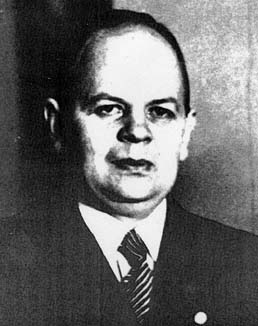
\includegraphics[height=3cm]{img/ackermann.jpg}\\
	Wilhelm \textbf{Ackermann}
\end{center}
} &
\parbox[t]{5cm}{
	\begin{center}
	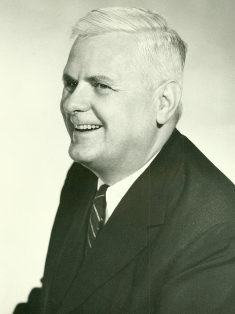
\includegraphics[height=3cm]{img/church.jpg}\\
		Alonzo \textbf{Church}
	\end{center}
} &
\parbox[t]{5cm}{
	\begin{center}
	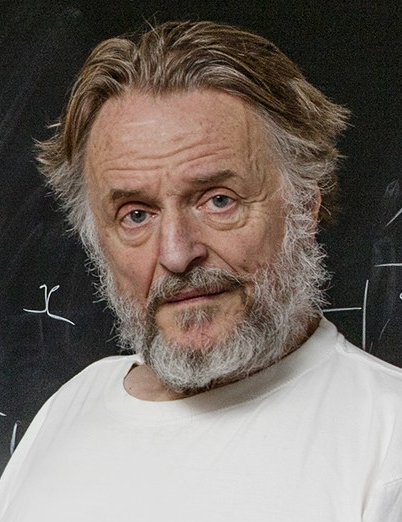
\includegraphics[height=3cm]{img/conway.jpg}\\
		John \textbf{Conway}
	\end{center}
} \\

\parbox[t]{5cm}{
	\begin{center}
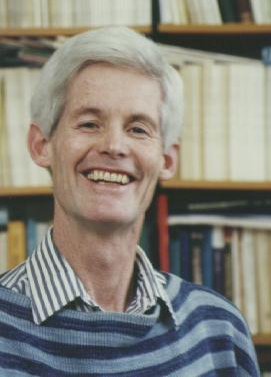
\includegraphics[height=3cm]{img/cook.jpg}\\
	Stephen \textbf{Cook}
	\end{center}
} &
\parbox[t]{5cm}{
	\begin{center}
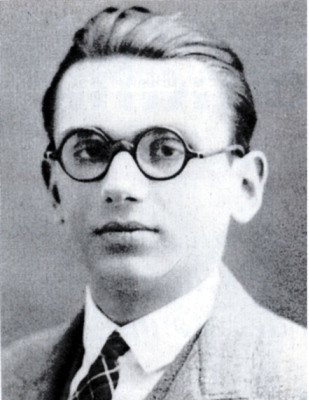
\includegraphics[height=3cm]{img/goedel.jpg}\\
	Kurt \textbf{Gödel}
	\end{center}
} &
\parbox[t]{5cm}{
	\begin{center}
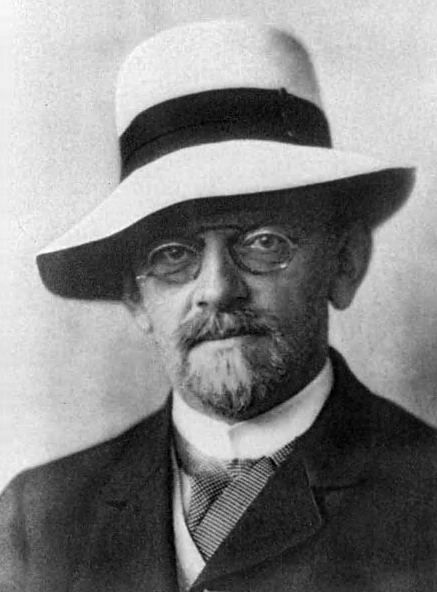
\includegraphics[height=3cm]{img/hilbert.jpg}\\
	David \textbf{Hilbert}
	\end{center}
} \\

\parbox[t]{5cm}{
	\begin{center}
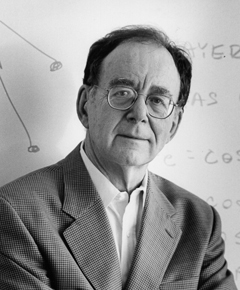
\includegraphics[height=3cm]{img/karp.jpg}\\
	Richard \textbf{Karp}
	\end{center}
} &
\parbox[t]{5cm}{
	\begin{center}
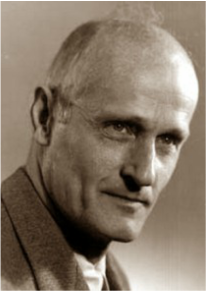
\includegraphics[height=3cm]{img/kleene.png}\\
	Stephen \textbf{Kleene}
	\end{center}
} &
\parbox[t]{5cm}{
	\begin{center}
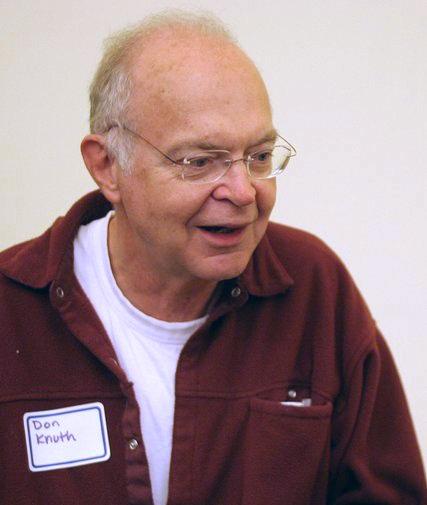
\includegraphics[height=3cm]{img/knuth.jpg}\\
	Donald \textbf{Knuth}
	\end{center}
} \\
\parbox[t]{5cm}{
	\begin{center}
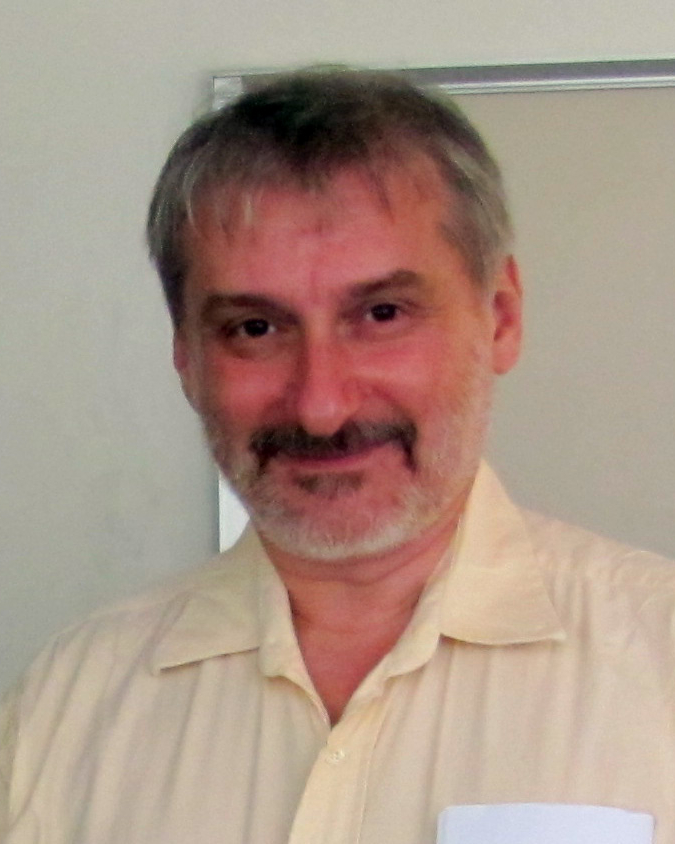
\includegraphics[height=3cm]{img/levin.jpg}\\
	Leonid \textbf{Levin}
	\end{center}
} &
\parbox[t]{5cm}{
	\begin{center}
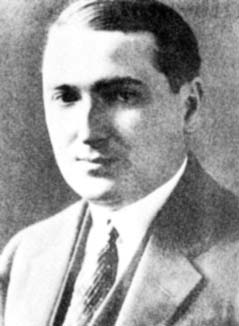
\includegraphics[height=3cm]{img/post.jpg}\\
	Emil \textbf{Post}
	\end{center}
} &
\parbox[t]{5cm}{
	\begin{center}
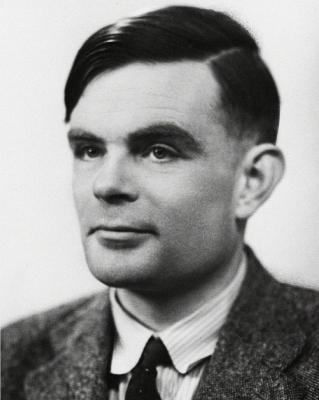
\includegraphics[height=3cm]{img/turing.jpg}\\
	Alan \textbf{Turing}
	\end{center}
}   
\end{tabular}
\end{adjustbox}
\end{document}
